\documentclass[twoside,letterpaper,twocolumn]{article}

%%%%%%%%%%%%%%%%%%%%%%%%%%%%%%%%%%%%%%%%%%%%%%%%%%%%%%%%%%%%%%%%%%%%%%
% Package with format specifications for the 9th CISBGf
\usepackage{cisbgf}


% \usepackage{natbib}
% Para portugues
\usepackage[latin1]{inputenc}
\usepackage{amsmath}
\usepackage{textcomp}
% \usepackage{endfloat}
% \usepackage{fixltx2e}
% \usepackage{stfloats}

%%%%%%%%%%%%%%%%%%%%%%%%%%%%%%%%%%%%%%%%%%%%%%%%%%%%%%%%%%%%%%%%%%%%%%
% MANDATORY PARAMETERS

% Setting the title
\title{3D gravity inversion by planting anomalous densities}

% Setting the authors
\author{Leonardo Uieda, Val�ria C. F. Barbosa (Observat�rio Nacional, Rio de Janeiro, Brazil)}

% Setting the headings
\headauthor{L. Uieda, V.C.F. Barbosa}
\headtitle{3D gravity inversion by planting anomalous densities}


%%%%%%%%%%%%%%%%%%%%%%%%%%%%%%%%%%%%%%%%%%%%%%%%%%%%%%%%%%%%%%%%%%%%%%
%%%%%%%%%%%%%%%%%%%%%%%%%%%%%%%%%%%%%%%%%%%%%%%%%%%%%%%%%%%%%%%%%%%%%%
\begin{document}

\maketitle

\begin{abstract}

This paper presents a novel gravity inversion method for estimating a 3D density-contrast
distribution defined on a grid of prisms. Our method consists of
an iterative algorithm that does not require the solution of a large equation system.
Instead, the solution grows systematically around user-specified prismatic elements
called ``seeds''. Each seed can have a different density contrast, allowing the
interpretation of multiple bodies with different density contrasts and interfering
gravitational effects. The compactness of the solution around the seeds is imposed
by means of a regularizing function.
The solution grows by the accretion of neighboring prisms of the current solution. The prisms
for the accretion are chosen by systematically searching the set of current neighboring
prisms. Therefore, this approach allows that the columns of the Jacobian matrix be
calculated on demand. This is a known technique from computer science called
``lazy evaluation'', which greatly reduces the demand of computer memory and processing
time. Test on synthetic data and on real data collected over the ultramafic Cana Brava
complex, central Brazil, confirmed the ability of our method in detecting sharp and
compact bodies.

\end{abstract}

\section{Introduction}

Over the past 20 years, substantial effort has been directed toward estimating
3D density-contrast distributions using gravity data inversion. Usually the inversion
methods, like that of Li and Oldenburg (1998), produce blurred images of anomalous
sources. On the other hand, methods for producing sharp images have been developed
by Portniaguine and Zhdanov (2002) and Silva Dias \textit{et al}. (2009). All
previously mentioned methods require the solution of large linear systems, which can
be computationally challenging for large problems. Attempts to overcome this problem
include: the method of Ren� (1986) that obtains 2D sharp and compact bodies by successively
incorporating cells around pre-specified cells called ``seeds'' with known density
contrasts; and the method of Camacho \textit{et al}. (2000) that recovers sharp 3D
bodies by means of a systematic search algorithm. We present a new 3D gravity inversion
that uses ``seeds'' around which the density anomalies grow, as in Ren� (1986), and
imposes compactness of the solution using a regularizing function like that of Silva
Dias \textit{et al}. (2009). Tests on synthetic data and on field data collected over
the ultramafic Cana Brava complex, Central Brazil, confirmed the potential of the method in
producing sharp images of the density anomalies.

\section{Forward modeling}

Consider a data set composed of $N$ observations of a gravity anomaly. We
assume that these observations are due to density anomalies confined in a three-dimensional
region of the subsurface. Let us consider that this region is divided into a set of $M$
juxtaposed right rectangular prisms. It follows that the gravitational attraction caused
by the density anomalies can be approximated by the sum of the contribution of each
prism, which can be calculated using the formulas of Nagy \textit{et al}. (2000).
Assuming that each prism has a constant density contrast, it follows that the relationship
between the vertical component of the gravitational attraction and the density contrast of
each prism is linear and can be expressed in matrix notation as
\begin{equation}
\mathbf{d} = \mathbf{G}\mathbf{p},
\label{eq:forward}
\end{equation}
where $\mathbf{d}$ is the data vector containing the vertical component of the gravitational
attraction caused by the prism ensemble, $\mathbf{p}$ is the parameter vector
containing the density contrast of each prism, and $\mathbf{G}$ is the Jacobian matrix
of the functional relation between $\mathbf{d}$ and $\mathbf{p}$.

\section{Inverse problem}

The inverse problem of estimating $\mathbf{p}$ is an ill-posed problem and thus requires
additional constraints to be solved. The constraints used in our method impose that the solution be
compact and concentrated around ``seeds'', which are user-specified prisms with known density
contrasts. These conditions can be imposed by means of a regularizing function in a similar
manner to Silva Dias \textit{et al}. (2009). Following this approach, we formulate the inverse
problem as minimizing the goal function
\begin{equation}
\Gamma(\mathbf{p}) = \phi(\mathbf{p}) + \mu \theta(\mathbf{p}),
\label{eq:goal}
\end{equation}
where $\mu$ is a regularizing parameter. Function $\phi(\mathbf{p})$ is a measure of
the data misfit, i.e., the $\ell_2$ norm of the residuals
\begin{equation}
\phi(\mathbf{p}) = ||\mathbf{d}^{o} - \mathbf{d}||_2 =
\sum\limits_{i=1}^{N} (d^{o}_i - d_i)^2,
\label{eq:misfit}
\end{equation}
where $\mathbf{d}^{o}$ is a vector containing the measured data and $\mathbf{d}$ is given by
equation \ref{eq:forward}.
Function $\theta(\mathbf{p})$ is a regularizing
function that enforces the compactness of the solution around the seeds and is similar
to that of Silva Dias \textit{et al}. (2009)
\begin{equation}
\theta(\mathbf{p}) = \sum\limits_{i=1}^{M} \dfrac{p_i}{p_i + \epsilon} l_i^{\beta},
\end{equation}
where $p_i$ is the $i$th element of $\mathbf{p}$, $\epsilon$ is a small and positive constant
used to avoid discontinuities, $l_i$ is the distance between the $i$th prism and the seed
to which it will be accreted, and $\beta$ is the power to which $l_i$ is raised and
controls the compactness of the solution.

\section{Algorithm}

Our algorithm requires a set of $N_S$ seeds specified by the user beforehand. These
seeds should be chosen according to prior information about the density anomalies,
such as geologic models, well logs and previous inversions. Each seed consists of a
prism of the interpretative model and thus the $s$th seed is described by a density
contrast value $\rho_s$ and a position index $i_s$ in the parameter vector.
The algorithm starts with an initial estimate $\mathbf{p}^0$ with all elements set
to zero. Next, the seeds are included in the initial estimate by setting
$p^0_{i_s} = \rho_s$. An iteration of the algorithm consists of trying to grow each
of the $N_S$ seeds by performing the accretion of one of its neighboring prisms. The
accretion of a prism to the $s$th seed is performed in three steps:
\begin{enumerate}
  \vspace{-0.3cm}
  \item Each neighboring prism of the seed is temporarily added to the estimate,
        one at a time, and the goal function $\Gamma$ (equation \ref{eq:goal}) is
        evaluated for the current
        estimate including the neighbor. Each neighbor is added to the estimate with
        the density contrast $\rho_s$ of the $s$th seed.
  \vspace{-0.3cm}
  \item One of the tested neighbors is chosen that both reduces the data-misfit function
        $\phi$ (equation \ref{eq:misfit}) and provides the smallest value of the
        goal function $\Gamma$ (equation \ref{eq:goal}). This chosen
        neighbor is then added permanently to the estimate, finalizing the accretion.
        If none of the neighboring prisms of the $s$th seed meet these criteria then
        the $s$th seed doesn't grow in this iteration.
  \vspace{-0.3cm}
  \item In the case that a neighboring prism is accreted to the $s$th seed, its neighboring prisms
        are appended to the seed's current neighbor list and the values of the goal and
        data-misfit functions are updated.
  \vspace{-0.3cm}
\end{enumerate}
These three accretion steps are repeated for each seed. After all seeds have tried to
grow a new iteration is started. This process stops when none of the seeds are
able to grow, signifying that the data-misfit function (equation \ref{eq:misfit})
cannot decrease any further. Figure \ref{fig:scheme} shows a 2D sketch of three stages of the
algorithm: the starting configuration; the end of the first iteration; and the final solution.

One of the main advantages of our algorithm is that it does not require the solution of
an equation system. Even more importantly, the full Jacobian matrix $\mathbf{G}$ is
not needed at any one time since the search is limited to neighboring prisms of the
current solution. This means that each column of $\mathbf{G}$ only needs to be calculated
when the prism of the interpretative model to which it refers becomes a neighbor of the
current solution. This technique is known in computer science as ``lazy evaluation''.
Furthermore, once a neighboring prism is permanently added to the solution, it's corresponding
column is no longer needed and can be discarded.
This results in fast inversion times and low memory usage, allowing the inversion of large
data sets using fine meshes without the need for supercomputers or data compression algorithms
(Portniaguine and Zhdanov, 2002).

\begin{figure*}[h]
    \centering
        \includegraphics[width=\textwidth]{scheme.png}
    \caption{2D sketch of three stages of the algorithm. \textbf{a)} Starting configuration
    using two seeds (dark red and dark green prisms). The neighbors
    of the red and green seeds are shown in light red and light green, respectively.
    \textbf{b)} State of the solution after the first iteration. \textbf{c)} The final
    result of the inversion after the algorithm stops showing compact bodies.
    \label{fig:scheme}}
\end{figure*}

\section{Application to synthetic data}

Synthetic gravity data (Figure \ref{fig:synth-data}a) was used to test the
performance and correctness of our method.
The data was calculated at
$z=0\ \text{km}$ and a Gaussian
error with standard deviation $0.5\ \text{mGal}$ and zero mean was added to the data to simulate
measurement errors.
The data was generated from the prismatic model shown in Figure \ref{fig:synth-res}a.
This model consists of two outcropping prismatic bodies with different sizes and density contrasts
of $0.3\ \text{g.cm}^{-3}$ and $0.4\ \text{g.cm}^{-3}$. 
A total of 87 seeds were used, all located at 500 m depth.
The interpretative model is composed of 50,000 juxtaposed rectangular prisms and the data set
totaled 1,250 measurements.

The final solution in Figure \ref{fig:synth-res}b clearly shows
that our method is able to recover the geometry of both prismatic bodies, despite their
strongly interfering gravitational effects. Figure \ref{fig:synth-res}c shows
the location of the seeds inside the final result.
The adjustment of the data predicted by the inversion to the synthetic data is shown in
Figure \ref{fig:synth-data}b.
It is noticeable that the data predicted by the inversion fits very closely to the synthetic,
noise-corrupted data. 

\begin{figure}[htb]
    \centering
        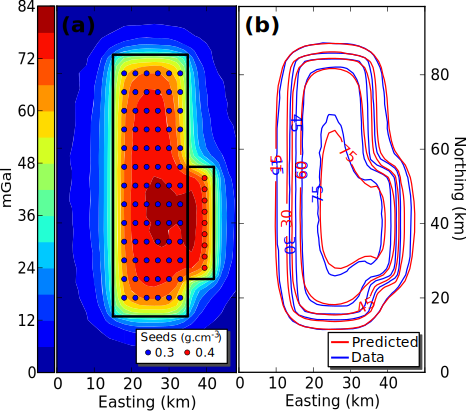
\includegraphics[width=8cm]{synthetic/data_seeds_adjustment.png}
    \caption{Test using noise-corrupted synthetic data. \textbf{a)} Synthetic data
    shown in a color map. Black lines denote the contour of the outcropping portion of
    the prismatic model. The seeds used in the inversion are represented by blue and red
    circles.
    \textbf{b)} Fit of the data predicted by the inversion (red lines) against the
    noise-corrupted synthetic data (blue lines).
    \label{fig:synth-data}}
\end{figure}

\begin{figure*}[h]
    \centering
        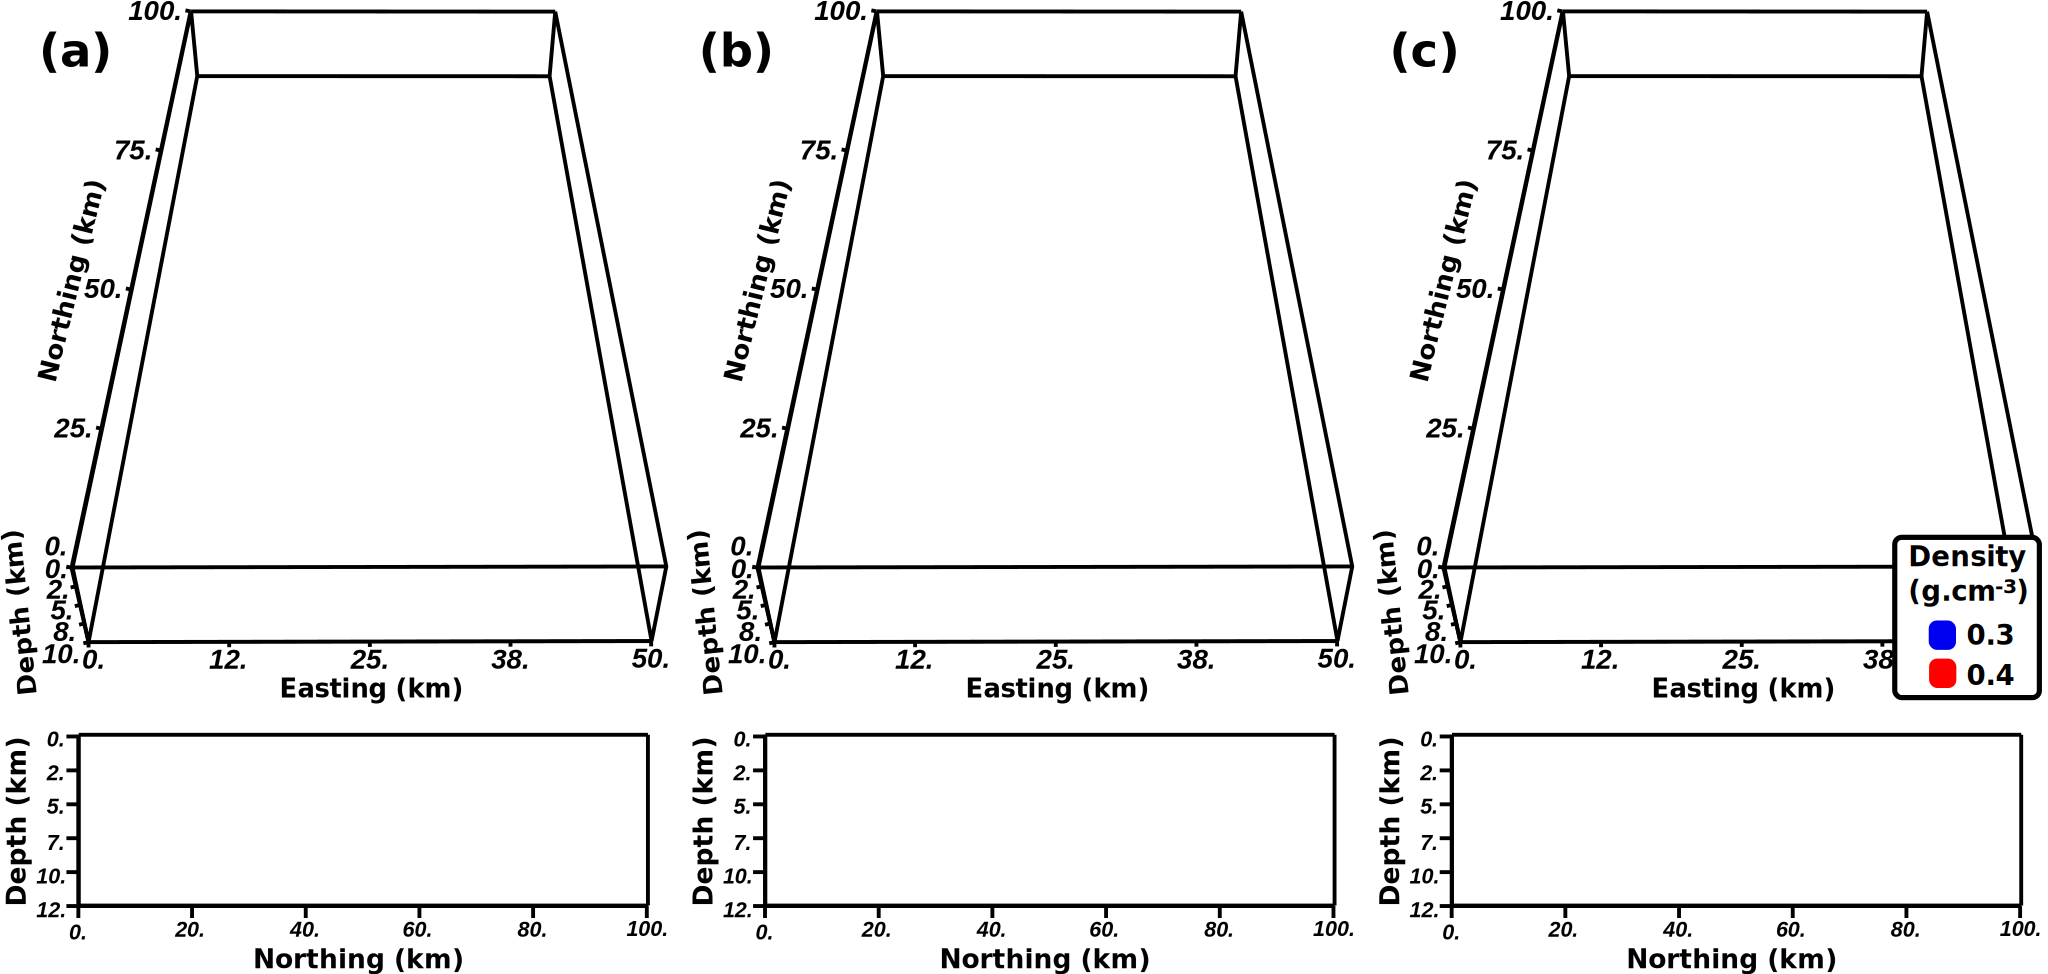
\includegraphics[width=\textwidth]{synthetic/results_all.png}
    \caption{Results of the test using noise-corrupted synthetic data.
    \textbf{a)} Model composed of two juxtaposed and outcropping rectangular prisms.
    The prism shown in blue has a thickness of 8 km while the one in red has
    6 km.
     \textbf{b)} Final result of the inversion. The contour of the synthetic model
     is shown in black lines for comparison.
     \textbf{c)} Seeds used in the inversion shown in dark red and dark blue.
     The estimated density-contrast distribution is shown with transparency for
     comparison.
    \label{fig:synth-res}}
\end{figure*}

\section{Application to field data}

We applied our inversion algorithm to gravity data collected over the outcropping
Cana Brava layered mafic-ultramafic complex (CBC) and the Palmeir�polis
volcano-sedimentary sequence (PVSS).
The CBC and PVSS are located within the Tocantins Province in central
Brazil, between the Amazonian and S�o Francisco cratons (Silva Dias \textit{et al}., 2009).
Figure \ref{fig:geomap} shows a simplified geologic map of the CBC and
PVSS and adjacent regions after Carminatti \textit{et al}. (2003).
The main host rock consists of metasedimentary sequences of the Serra da
Mesa Group. Figure \ref{fig:canabrava-data}a shows the residual Bouguer anomaly map over
the CBC and PVSS bodies. Carminatti \textit{et al}. (2003) interpret the CBC as having a density contrast of
$0.39\ \text{g.cm}^{-3}$ and the PVSS of $0.27\ \text{g.cm}^{-3}$. These values were used to generate
a set of seeds at $z=0\ \text{km}$ concentrated inside the outline of the outcrop. A second
set of seeds located at $z=2\ \text{km}$ was used for the PVSS only. The seeds are shown in
Figure \ref{fig:canabrava-data}a along with the outline of the outcropping portion
of the CBC and PVSS. The data set is composed of 132 measurements, the interpretative model
has 432,937 prisms and the total number of seeds is 269. When performed on a computer with an
Intel\textregistered$\ $ Core\texttrademark$\ $ 2 Duo P7350 2.0 GHz processor, the total
time for the inversion was approximately 3.75 minutes.

The result of the inversion is shown in Figure \ref{fig:canabrava-res} and is in
agreement with previous interpretations by Silva Dias \textit{et al}. (2009).
The adjustment of the data predicted by the inversion to the observed gravity data is shown in
Figure \ref{fig:canabrava-data}b. The fit is very close for areas where there is data
(shown as $+$ symbols) and worse for areas where data is lacking. This is expected and is
most likely a product of the interpolation used for generating the contour plot.

\begin{figure}[htb]
    \centering
        \includegraphics[width=8cm]{cana-brava/geologic_map_canabrava.png}
    \caption{Simplified geologic map of the CBC and PVSS and adjacent regions, after
    Carminatti \textit{et al}. (2003).
    \label{fig:geomap}}
\end{figure}

\begin{figure}[htb]
    \centering
        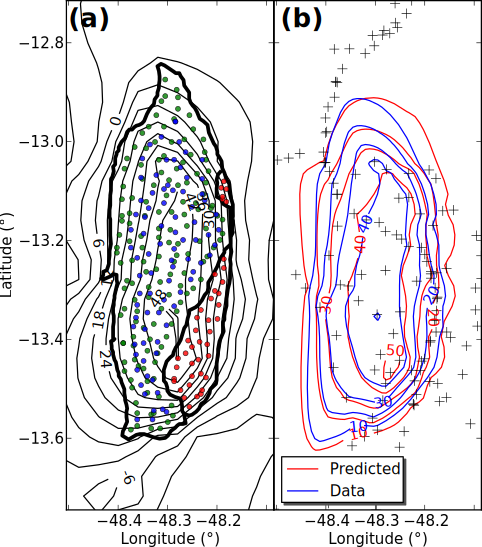
\includegraphics[width=8cm]{cana-brava/seeds_adjustment.png}
    \caption{Gravity data of the Cana Brava complex.
    \textbf{a)} Residual Bouguer anomaly map, contour of the outcropping portion (black lines),
    and seeds used in the inversion (blue, green, and red circles). Seeds shown in blue and
    green have a density contrast of $0.27\ \text{g.cm}^{-3}$ and the ones shown in red have
    $0.39\ \text{g.cm}^{-3}$. Seeds in blue and red where placed at $z=0\ \text{km}$
    and seeds in green at $z=2\ \text{km}$.
    \textbf{b)} Fit of the data predicted by the inversion (red lines) against the residual
    Bouguer anomaly map (blue lines). Data points are shown as $+$ symbols.
    \label{fig:canabrava-data}}
\end{figure}

\begin{figure*}[h]
    \centering
        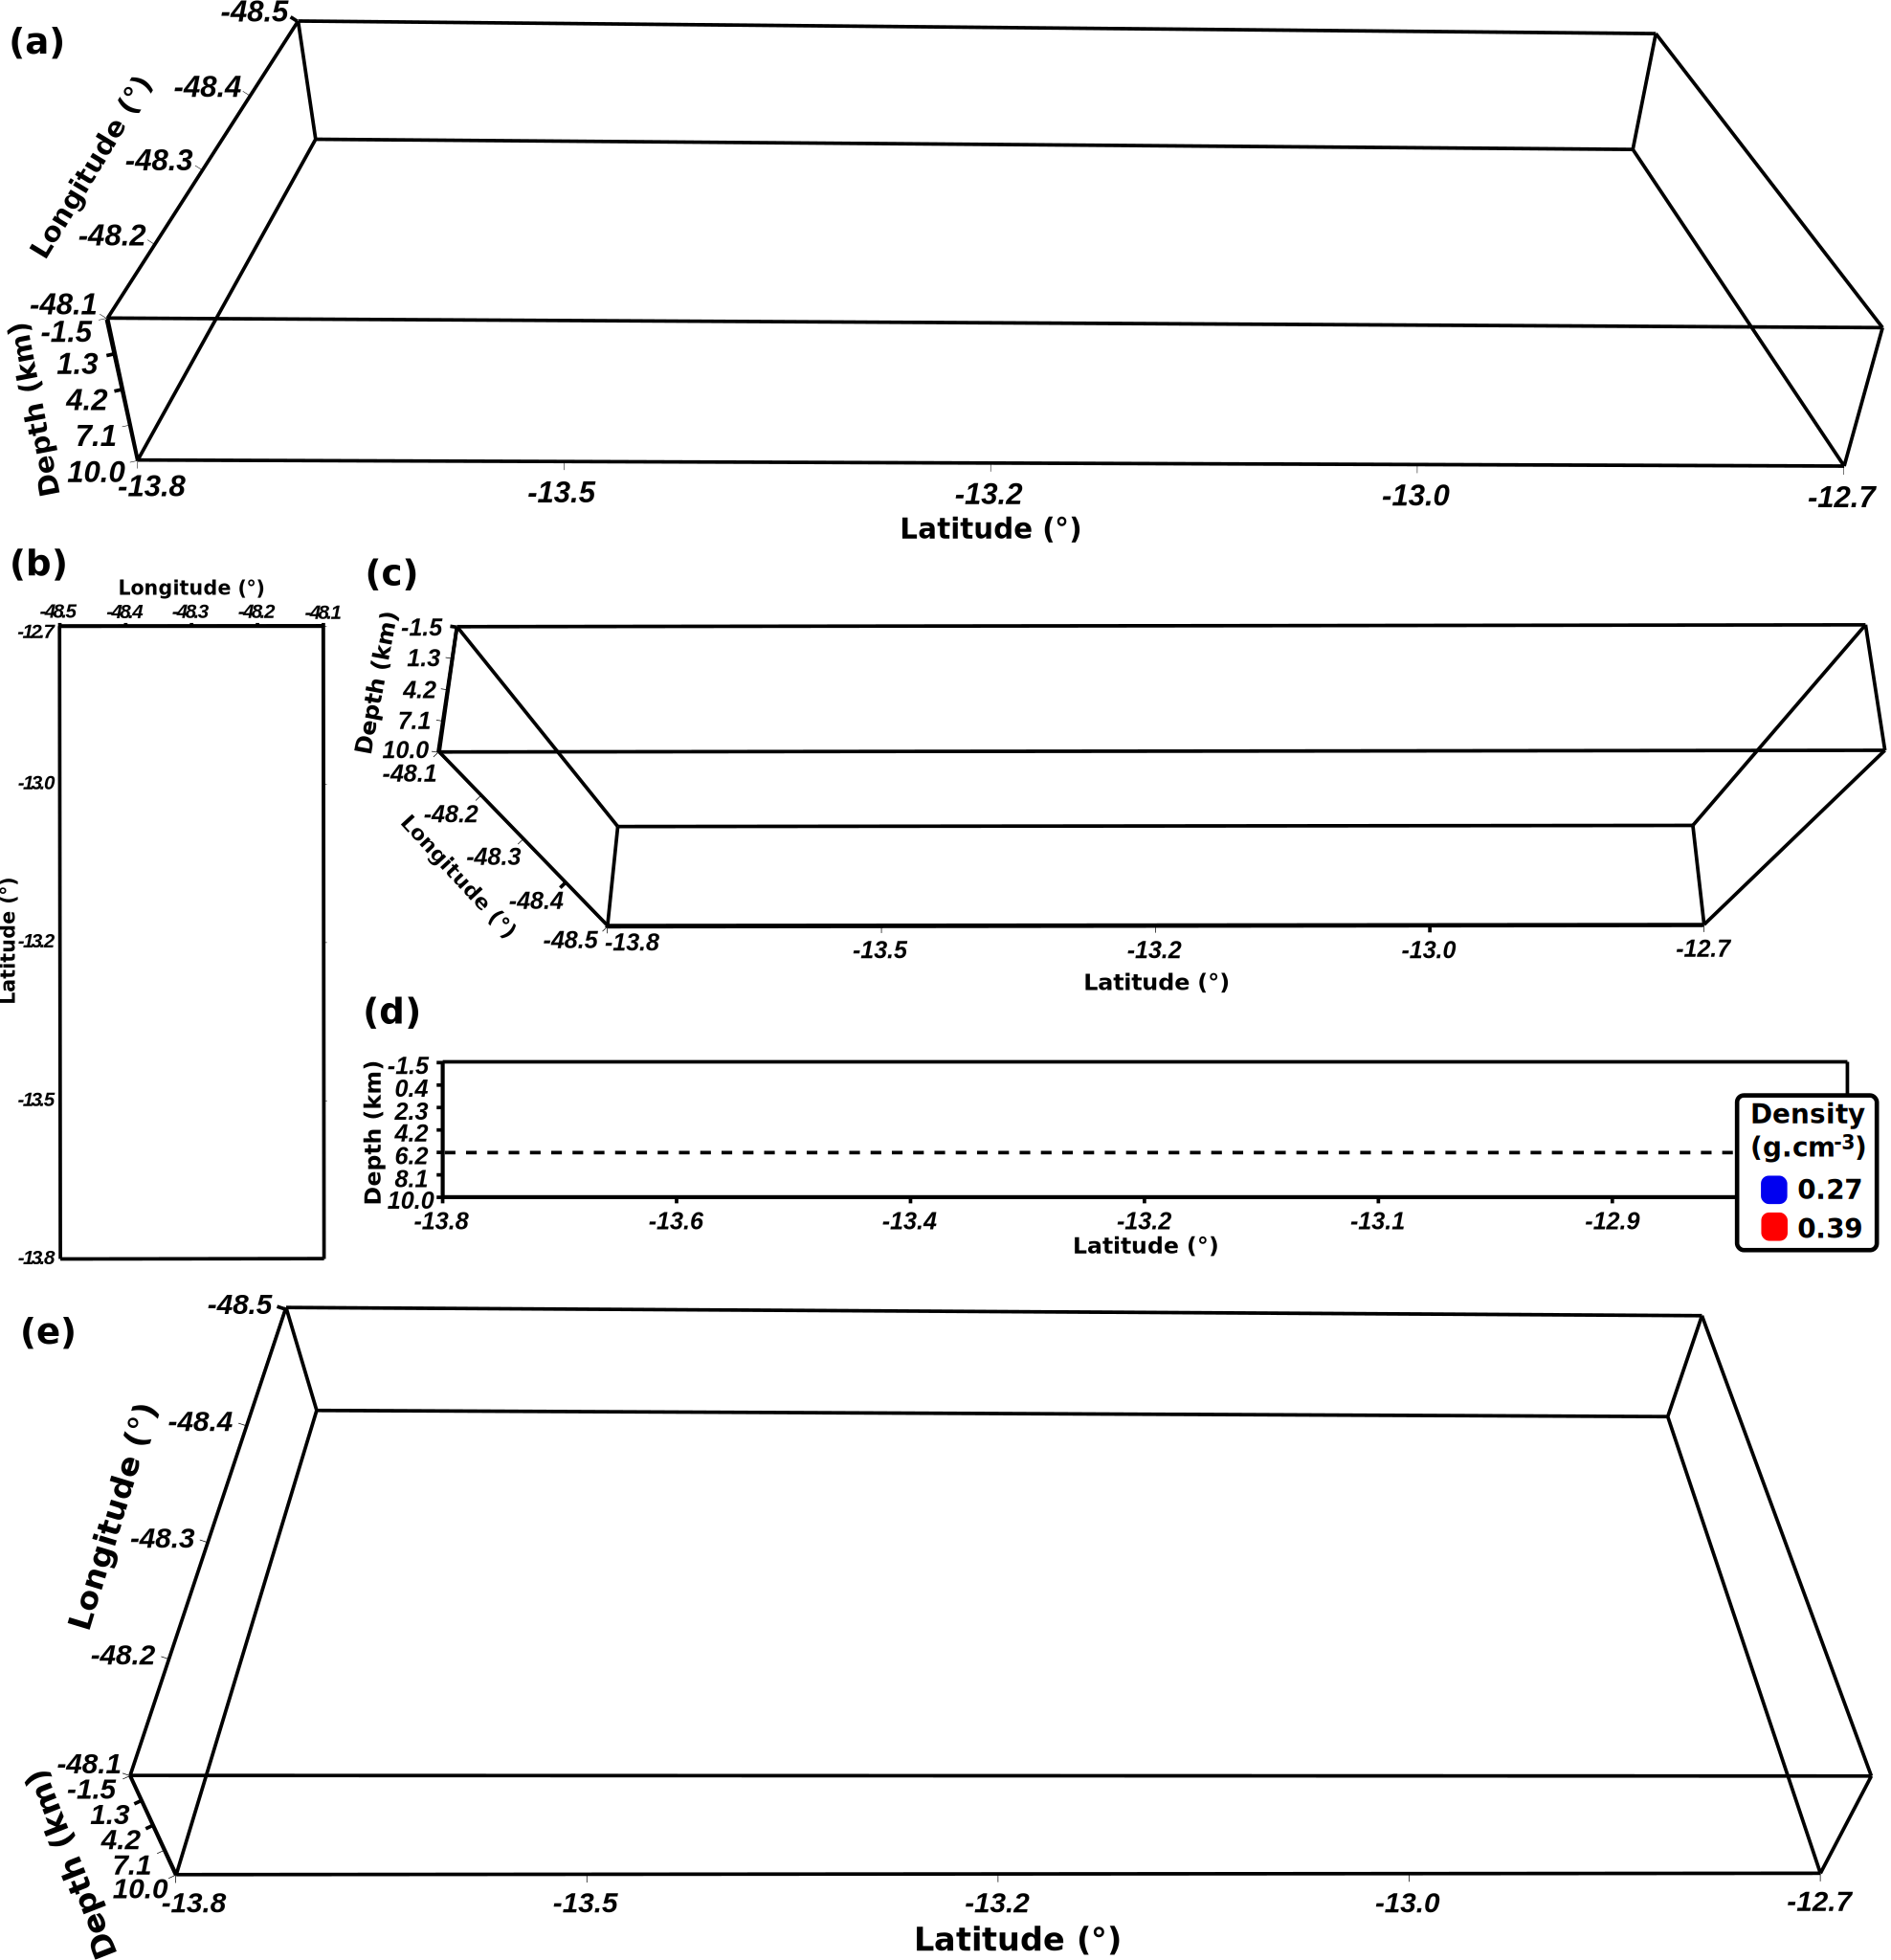
\includegraphics[width=17.5cm]{cana-brava/result.png}
    \caption{Result of the inversion of the Cana Brava complex gravity data.
    \textbf{a-d)} The estimated density-contrast distribution in different views.
    The maximum depth of the PVSS was approximately 6 km.
    \textbf{e)} Seeds used in the inversion shown in dark blue and dark red.
    \label{fig:canabrava-res}}
\end{figure*}

\section{Conclusions}

We have presented a new method for linear 3D inversion of gravity data that is based on a
systematic search algorithm. Prior information is incorporated into the solution by means
of prismatic elements called ``seeds'' around which the solution is concentrated.
Large data sets and fine interpretative models can be easily handled by implementing
a ``lazy evaluation'' of the Jacobian matrix.
Synthetic and field data tests show that our method is able to recover compact bodies
with different density contrasts that produce strongly interfering gravitational effects.
The results obtained for the Cana Brava complex are in agreement with previous interpretations.

\section{References}

Camacho, A. G., Montesinos, F. G. and Vieira, R., 2000, Gravity inversion by
means of growing bodies: Geophysics, Vol. 65, No. 1, p95-101.

Carminatti, M. G., Marangoni, Y. R., Correia, C. T., 2003, Modelagem
gravim�trica do complexo de Cana Brava e sequ�ncia de Palmeir�polis,
GO: Revista Brasileira de Geoci�ncias, Vol. 33, p245-254.

Li, Y., Oldenburg, D. W., 1998, 3-D inversion of gravity data: Geophysics, Vol. 63,
No .1, p109-119.

Nagy, D., Papp, G., Benedek, J., 2000, The gravitational potential and its
derivatives for the prism: Journal of Geodesy, Vol. 74, p552-560.

Portniaguine, O., Zhdanov, M. S., 2002, 3-D magnetic inversion with data compression
and image focusing: Geophysics, Vol. 67, No. 5, p1532-1541.

Ren�, R. M., 1986, Gravity inversion using open, reject, and ``shape-of-anomaly'' fill
criteria: Geophysics, Vol. 51, No. 4, p988-994.

Silva Dias, F. J. S., Barbosa, V.C.F., Silva, J.B.C, 2009, 3D gravity inversion through an
adaptive-learning procedure: Geophysics, Vol. 74, No. 3, pI9-I21.

\section{Acknowledgments}

This research is supported by the Brazilian agencies CNPq and CAPES.
We thank Y�ra Regina Marangoni for the gravity data over the Cana Brava complex.

\clearpage

\end{document}
